\textbf{Задача №77381 тип №6}

\begin{figure}[h]
	\centering
	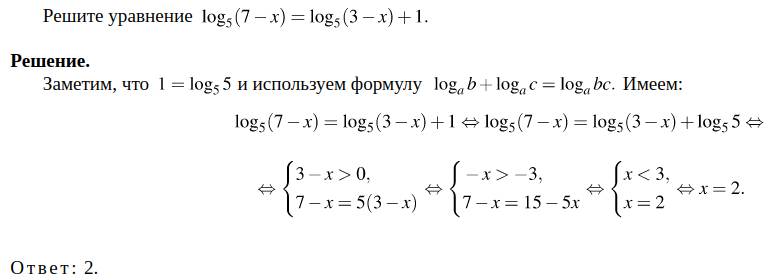
\includegraphics[width=1\linewidth]{VM/god.png}
\end{figure}

Первая часть шаблона задачи №77381
 
Здесь, помимо ввода переменных, и подбора подходящего корня, происходит проверка корня на его вхождение в ОДЗ, а также проверяется сколько знаков после запятой он имеет. В данном случае, программа контролирует, чтобы ответ имел не более 3 знаков. Сделано это, чтобы пользователю было удобнее вводить ответ.

\lstinputlisting{paragrafs/Zadachi/5}

Вторая часть шаблона задачи №77381

Ещё одной отличительной особенностью этого шаблона, является его библиотека \texttt{setAdditiveEquationTask}. Благодаря ней, части уравнения, записанные в квадратные скобки после слова \texttt{parts:} будут каждый раз переставлятся при запуске программы, что создаёт больше разнообразия в задачах, использующих этот код.

Эта часть также содержит некоторые специальные встроенный функции:
\\ \texttt{[a,b,c].slag()} – функция выводящая пример, в котором все элементы массива слагаемыми в различном порядке.
\\ \texttt{a.pow(b)} – функция возводящая число в степень
И некоторые команды из LaTeX, например: 
\\  \texttt{\textbackslash \textbackslash cdot} - выводящая знак умножения в виде точки.

\lstinputlisting{paragrafs/Zadachi/6}

\newpage

\textbf{Задачи сгенерированные по шаблону}

\begin{figure}[h]
	\centering
	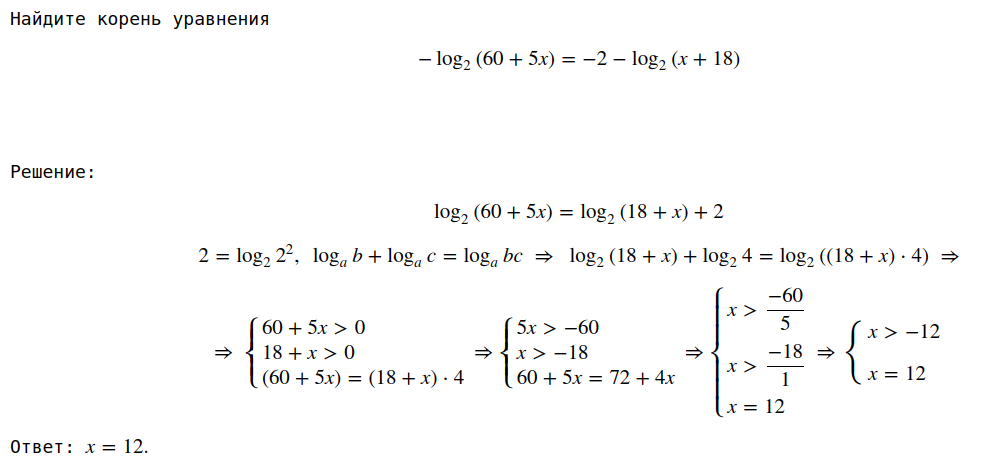
\includegraphics[width=1\linewidth]{VM/asd1.png}
	\end{figure}
	\begin{figure}[h]
	\centering
	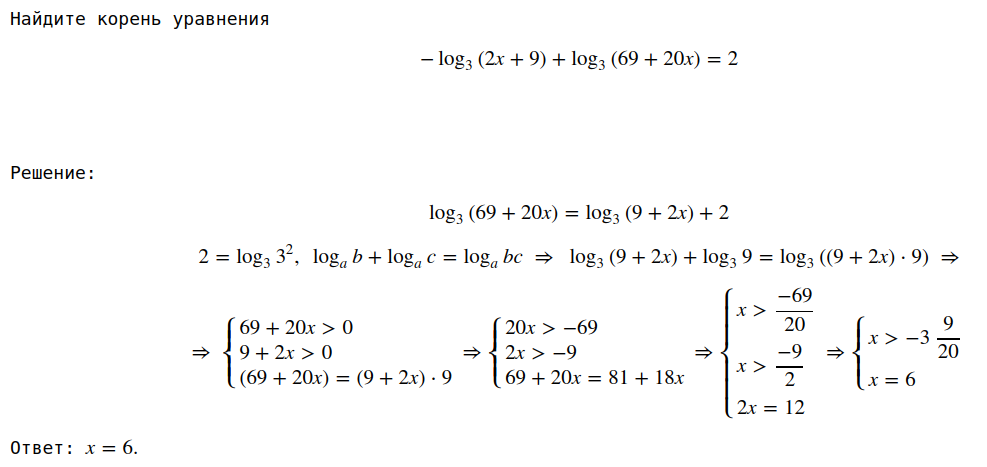
\includegraphics[width=1\linewidth]{VM/asd2.png}
\end{figure}
